\section{Parameter Identification}
\label{sec:methods:parameter_identification}

As we have introduced in Section \ref{sec:introduction:background:deep_probabilistic_methods}, different deep probabilistic methods are proposed for Bayesian parameter identification. In real applications, it is usually desired to identify the system parameters from multimodal observations. We start to introduce a universal framework with deep generative models for amortized Bayesian inference. This framework can be seen as a generalization of the BayesFlow \citep{radev2020bayesflow}.

\subsection{Universal Framework with Deep Generative Models for Amortized Bayesian Inference}
\citeauthor{radev2020bayesflow} \citeyearpar{radev2020bayesflow} proposed BayesFlow as an amortized Bayesian inference approach with normalizing flows. BayesFlow consists of a summary network for extracting information from the observations, and a conditional normalizing flow for learning the posterior distribution of parameters conditioned on the extracted information. This framework can be generalized to other deep generative models, such as \ac{VAE}, \ac{FM}, and diffusion models. Figure \ref{fig:universal_framework} illustrates the framework. We call the summary network here "condition network" to emphasize that the embeddings of observations function as condition in the \acp{DGM}. The major advantages of applying deep generative models as the Bayesian inference backbone are threefold:
\begin{itemize}
    \item \acp{DGM} consider the parameter identification as posterior inference, which provides naturally trustworthiness of the estimates;
    \item \acp{DGM} seek to model the posterior distribution on a large dataset, which is suitable for amortized Bayesian inference;
    \item compared with other architectures, like \acp{BNN}, \acp{DGM} achieve preciser posterior inference because of the separate inference and generation procedures.
\end{itemize}

In many generative tasks, such as text, image, and video generation, the condition is assumed to be simple. In contrast, for solving inverse problems, such as parameter identification, the generative model is supposed to "generate" variables under some complexer conditions. Thus, a well-designed condition network is essential to extract most informative features from the observations. This universal framework automatically encourages the condition network to deliver desirable embeddings to the deep generative model. Besides, each observation is only required to processed once while sampling the trained generative model for multiple times, which is computationally efficient. 

\begin{figure}[H]
    \centering
    \begin{minipage}[t]{0.49\textwidth}
        \centering
        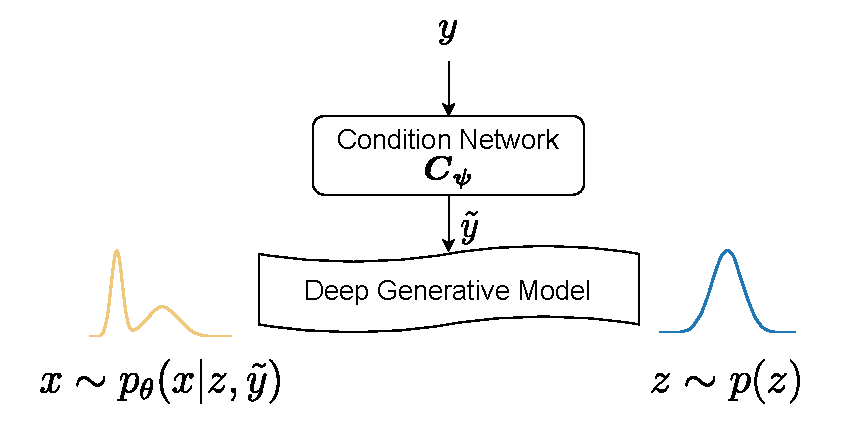
\includegraphics[width=\textwidth, valign=t]{figures/DGM_ABI.pdf}
        \caption[Universal Framework of Using Deep Generative Models for Amortized Bayesian Inference]{\small Universal Framework of Using Deep Generative Models for Amortized Bayesian Inference. The corresponding algorithm is shown on the right side (Algorithm \ref{alg:dgm_abi}). Training paradigms differ significantly across \acp{DGM}. While \acp{VAE} and \acp{NF} maximize the \ac{ELBO} and log-likelihood respectively, flow-based and diffusion models typically minimize a matching cost—regressing either a vector field (\acp{FM}), a score function, or added noise (\ac{DDPM}). Consequently, Bayesian inference is performed either via a direct deterministic mapping or by numerically integrating a differential equation (ODE or SDE).}
        \label{fig:universal_framework}
    \end{minipage}
    \hfill
    \begin{minipage}[t]{0.48\textwidth}
        \vspace{0pt}
        \begin{algorithm}[H]
            \caption{DGM-ABI Training \& Inference}
            \label{alg:dgm_abi}
            \begin{algorithmic}[1]
            \footnotesize % Reduce font size slightly to fit better
            \REQUIRE Dataset $\mathcal{D} = \{(x^{(i)}, y^{(i)})\}_{i=1}^M$
            \REQUIRE Prior $p(z)$, Condition network $C_\psi$
            \REQUIRE Generator $p_\theta(x \mid z, \tilde{y})$, (Optional: Inference $q_\phi(z \mid x, \tilde{y})$)
            
            \vspace{0.1cm}
            \STATE \textbf{Stage 1: Amortized Learning}
            \WHILE{not converged}
                \STATE Sample batch $\{(x, y)\} \sim \mathcal{D}$
                \STATE Compute embeddings: $\tilde{y} \leftarrow C_\psi(y)$
                \STATE Sample latent: $z \sim p(z)$
                \STATE Compute objective gradient:
                \STATE $g \leftarrow \nabla_{\theta,\psi,\phi} \, \mathcal{L}$
                \STATE Update parameters: $(\theta, \psi, \phi) \leftarrow (\theta, \psi, \phi) - \eta \cdot g$
            \ENDWHILE

            \STATE \textbf{Stage 2: Bayesian Inference}
            \STATE Given observed condition $y_{\text{obs}}$:
            \STATE $\tilde{y}_{\text{obs}} \leftarrow C_\psi(y_{\text{obs}})$
            \FOR{$k=1$ to $K$}
                \STATE Sample $z^{(k)} \sim p(z)$
                \STATE Generate $x^{(k)} \sim p_\theta(x \mid z^{(k)}, \tilde{y}_{\text{obs}})$
            \ENDFOR
            \RETURN Posterior samples $\{x^{(k)}\}_{k=1}^K$
            \end{algorithmic}
        \end{algorithm}
    \end{minipage}
\end{figure}

\subsection{Normalizing Flows for Parameter Identification}
Why are \acp{NF} more suitable for parameter identification tasks given time series observations? In this section, we will answer this question in terms of (1) inference accuracy and precision (2) reliability, i.e., whether the ground truth lies in the posterior, (3) speed, i.e., inference computational time, (4) sample efficiency, i.e., posterior contraction while increasing data amount, (5) correlation, i.e., identifying linearly correlated parameters, (6) complexity, i.e., handling multimodal distributions.

\paragraph{Overall Settings}
In this section, we take a classic mass-spring-damper system as an example, which has three parameters including mass $m$, spring constant $k$, and damping coefficient $c$. As observations, we take the position and velocity trajectories. For evaluation of (1) - (4), an external force is introduced. The \ac{ODE} is:
\begin{equation}
    \dot x = v,\; \dot v = \frac{1}{m}(F_t-kx-cv),\; F_t = 10\cdot sin(3t).
\end{equation}

For the (5) linear correlation case, the external force is removed, and the parameter $m$ and $k$ are correlated, i.e., $k=10\cdot m$. To investigate the (6) multimodal case, the system is extended into "Wall -- $k_1$ -- $m$ -- $k_2$ -- $m$ -- $k_3$ -- Wall". When the parameters $m$, $k_2$, and $c$ are fixed as constant, and we take the middle points of the positions and velocities of the two masses as observations, the value of $k_1$ and $k_3$ can not be uniquely distinguished. The \ac{ODE} becomes
\begin{align}
    \dot x_1 &= v_1,\;\dot v_1=\frac{1}{m}(-k_1x_1+k_2(x_2-x_1)-cv_1);\\
    \dot x_2 &= v_2,\;\dot v_2=\frac{1}{m}(-k_3x_2-k_2(x_2-x_1)-cv_2).
\end{align}

We compare two normalizing flow architectures \ac{RealNVP}, and \ac{NSF} with \ac{FM}, \ac{DDPM}, and \ac{SBM}, as well as \ac{VAE} and \ac{BNN}. As the condition network, we use an \ac{LSTM} layer followed by two linear layers with \ac{ELU} activations. For a group of estimated $\{ \widehat{x}^{(m)}\}_{m=1}^{M}$ and true parameters $ \{ x^{(m)}\}_{m=1}^{M}$ with the mean of the true parameters $\overline{x}$, the following evaluation metrics are applied:
\begin{itemize}
    \item Accuracy: \ac{RMSE} and R² score:
    \begin{equation}
        RMSE = \sqrt{\frac{1}{M}\sum_{m=1}^M (x^{(m)} - \widehat{x}^{(m)})^2}\;,
    \end{equation}
    \begin{equation}
        R^2 = 1 - \sum_{m=1}^{M}\frac{(x^{(m)}-\widehat{x}^{(m)})^2}{(x^{(m)}-\overline{x})^2}\;.
    \end{equation}

    \item Precision: \ac{MCIW}. For the $m$-th parameter by sampling it $L$ times, the standard deviation is $\sigma_{\widehat{x}^{(m)}}$, and we have:
    \begin{equation}
        CI^{(m)}(95\%)= [L_{m}, U_{m}] = \widehat{x}^{(m)}\pm 1.96\frac{\sigma_{\widehat{x}^{(m)}}}{\sqrt{L}}.
    \end{equation}
    Then the MCIW can be obtained by:
    \begin{equation}
        MCIW = \frac{1}{M}\sum_{m=1}^{M}(U_m - L_m).
    \end{equation}
    \item Reliability: \ac{CICP}. The larger \ac{CICP} indicates higher reliability of estimation.
    \begin{equation}
        CICP = \frac{1}{M}\sum_{m=1}^{M}c_m, \:
        c_m  = \begin{cases}
                0 & \text{ if } x ^{(m)} \notin [L_{m}, U_{m}], \\ 
                1 & \text{ otherwise. } 
              \end{cases}
    \end{equation}
\end{itemize}

\paragraph{Pperformance Comparison}
\begin{table}[ht]
    \centering
    \caption[Performance Benchmarking of Deep Bayesian Inference Methods]{Performance Benchmarking of Deep Bayesian Inference Methods on the Mass-Spring-Damper System. All metrics represent averages across the three system parameters. Predictive accuracy is assessed via RMSE (lower is better) and R² (higher is better). Uncertainty quantification is evaluated through the CICP and MCIW together. Ideal performance is characterized by a CICP near the 95\% calibration target; significantly lower values indicate overconfidence, while excessively high MCIW values indicate model imprecision. Inference time denotes the total computational time for a single test scenario based on 100 posterior samples.}
    \label{tab:metrics_005}
    \small
    \begin{tabular}{lccccc}
        \toprule
        \textbf{Model} & \textbf{RMSE} $\downarrow$ & \textbf{$R^2$} $\uparrow$ & \textbf{CICP} $\uparrow$ & \textbf{MCIW} $\downarrow$ & \textbf{Inference Time (s)} $\downarrow$ \\ 
        \midrule
        BNN     & 0.0393 & 0.9965 & 0.9900 & 0.1874 & 0.0209 \\
        VAE     & 0.0287 & \textbf{0.9987} & 0.7250 & \textbf{0.0497} & \textbf{0.0018} \\
        DDPM    & 0.0915 & 0.9852 & 0.9883 & 0.5338 & 0.2310 \\
        SBM     & 0.0699 & 0.9909 & 0.9700 & 0.3289 & 0.0534 \\
        FM      & 0.0547 & 0.9938 & \textbf{0.9933} & 0.3730 & 0.0050 \\
        RealNVP & \textbf{0.0278} & 0.9986 & 0.9917 & 0.1223 & 0.0043 \\
        NSF     & 0.0401 & 0.9966 & 0.9917 & 0.1845 & 0.0069 \\
        \bottomrule
    \end{tabular}
\end{table}

\begin{figure}[htp!]
    \begin{minipage}{0.7\textwidth}
        \centering
        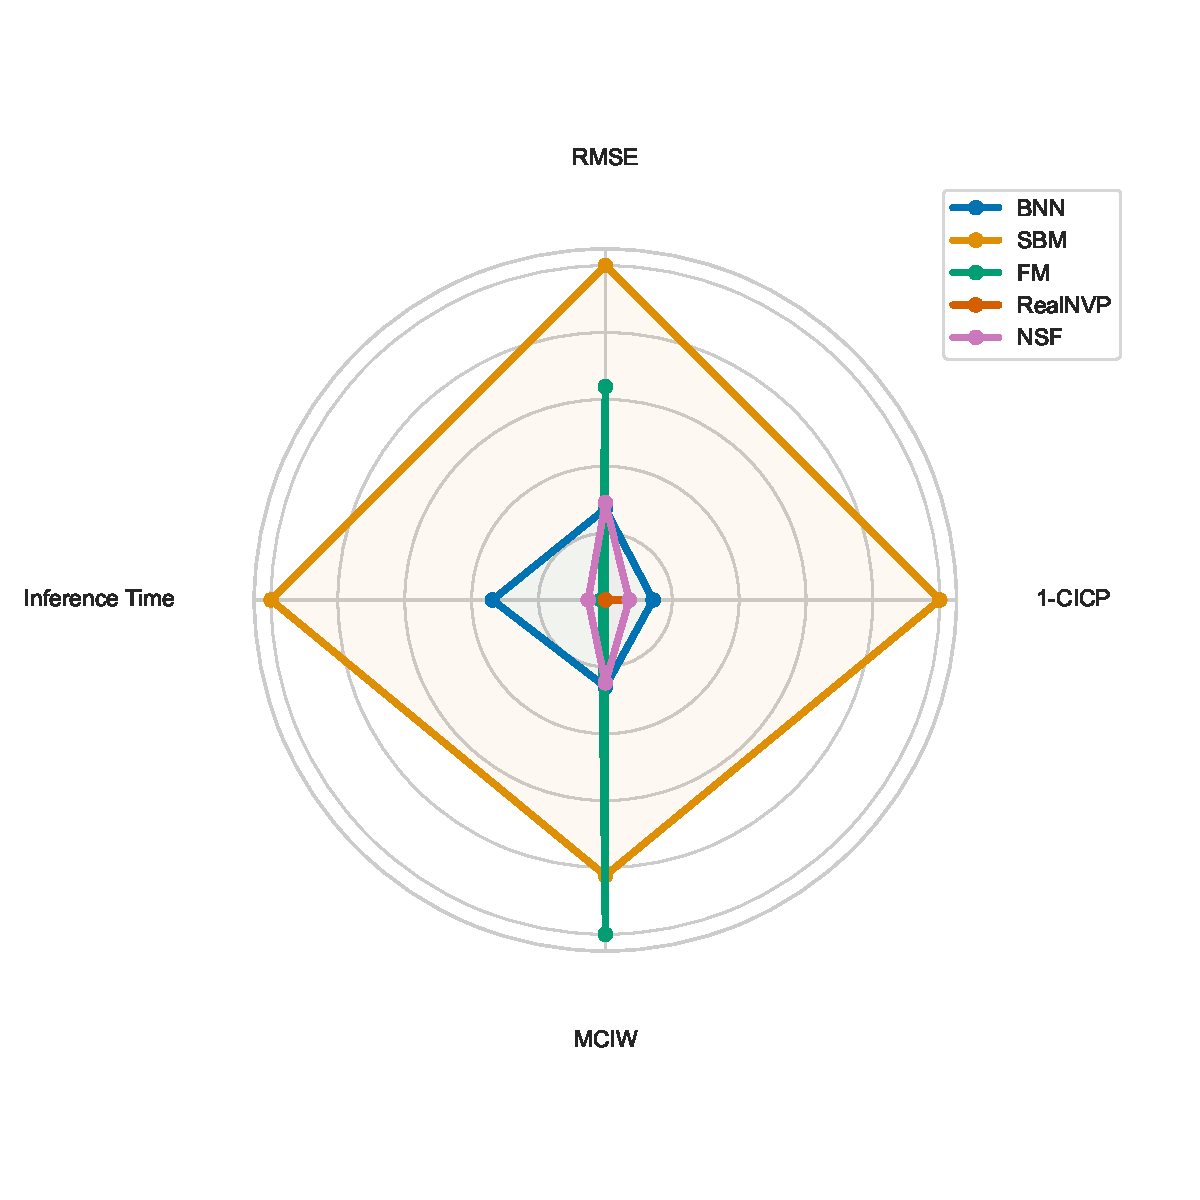
\includegraphics[width=\linewidth]{figures/metrics_0.05_spider_chart.pdf}
      \end{minipage}
      \hfill
    \begin{minipage}{0.28\textwidth}
    \caption[Detailed Comparison of Deep Bayesian Inference Methods]{Detailed Comparison of Deep Bayesian Inference Methods on the Mass-Spring-Damper System. The values are the same as those in Table \ref{tab:metrics_005}. "1-CICP" is shown for the sake of consistency of comparison, meaning that all metrics shown in the spider chart are "lower is better". The center of the radar plot represents optimal performance.}
    \label{fig:metrics_005_spider}
    \end{minipage}
\end{figure}

In Table \ref{tab:metrics_005} the evaluation of different models is shown. The observed time series are from $0\,s$ to $1\,s$ with the time step of $0.05\,s$, and no noises are added onto them. In terms of accuracy, \ac{RealNVP} (RMSE: 0.0278) and VAE (RMSE: 0.0287) are the most accurate models. Their highest R² scores indicate that they explain almost all the variance in the Mass-Spring-Damper system. \ac{DDPM} (RMSE: 0.0915) has the highest error in this group. While an R² of 0.985 is still objectively good, it is significantly less precise than the \acp{NF} (\ac{RealNVP}, \ac{NSF}) for this specific physical task. Overall, the flow-based methods (\ac{RealNVP}, \ac{NSF}, and \ac{FM}) achieve higher accuracy than diffusion-based methods (\ac{DDPM} and \ac{SBM}). The \ac{BNN} is comparable with the \acp{NF}.

In terms of uncertainty quantification, almost all models (except VAE) show CICP values near 1.0. Theoretically, the ideal CICP with 95\% confidence intervals should also be 0.95. Higher CICPs mean that they are conservative and under-confident, whereas the lower CICPs indicate overfitting. Besides, in an ideal noise-free scenario, the posterior distribution for the mass-spring-damper parameters should approach a Dirac delta function. However, in practice of solving inverse problems, the interval should never be zero. Because different parameters might produce very similar trajectories. Moreover, the models themselves have uncertainty due to limited data. Therefore, the CICPs higher than 0.95 mean that the inference models prioritize the reliability over precision.  Consequently, the MCIW should be considered together with CICP. \ac{VAE} (CICP: 0.7250 and MCIW: 0.0497) is overconfident. Its intervals are so narrow that the truth falls outside of them 27.5\% of the cases. \ac{DDPM} (CICP: 0.9883 and MCIW: 0.5338) is unprecise. It achieves high coverage simply by producing very wide intervals. 

In terms of computational efficiency, \ac{VAE} exhibits the highest inference speed. Flow-based methods demonstrate comparable performance to one another, though they are approximately $5\times$ slower than the \ac{VAE} baseline. \ac{BNN} follows, showing higher latency than the flow-based models but maintaining a clear advantage over \ac{SBM}. Finally, \ac{DDPM} is identified as the most computationally intensive approach, recording the slowest inference times.

With \ac{VAE} and \ac{DDPM} excluded due to miscalibration and computational overhead respectively, Figure \ref{fig:metrics_005_spider} visualizes the performance trade-offs of the remaining five architectures. \ac{RealNVP} exhibits the most optimal profile, represented by the smallest polygon area; it successfully minimizes \ac{RMSE} and \ac{MCIW} while maintaining near-perfect coverage. \ac{NSF} and \ac{FM} show comparable speed and accuracy but yield less precise (wider) credible intervals. The \ac{BNN} maintains high reliability (low 1-CICP) but suffers from increased inference time. Finally, \ac{SBM} shows the least favorable performance, characterized by the largest predictive error, the widest uncertainty bounds, and the longest computational time, indicating a difficulty in parameter identification compared to flow-based alternatives. 

\paragraph{Sample Efficiency}
\begin{figure}[htp!]
    \centering
    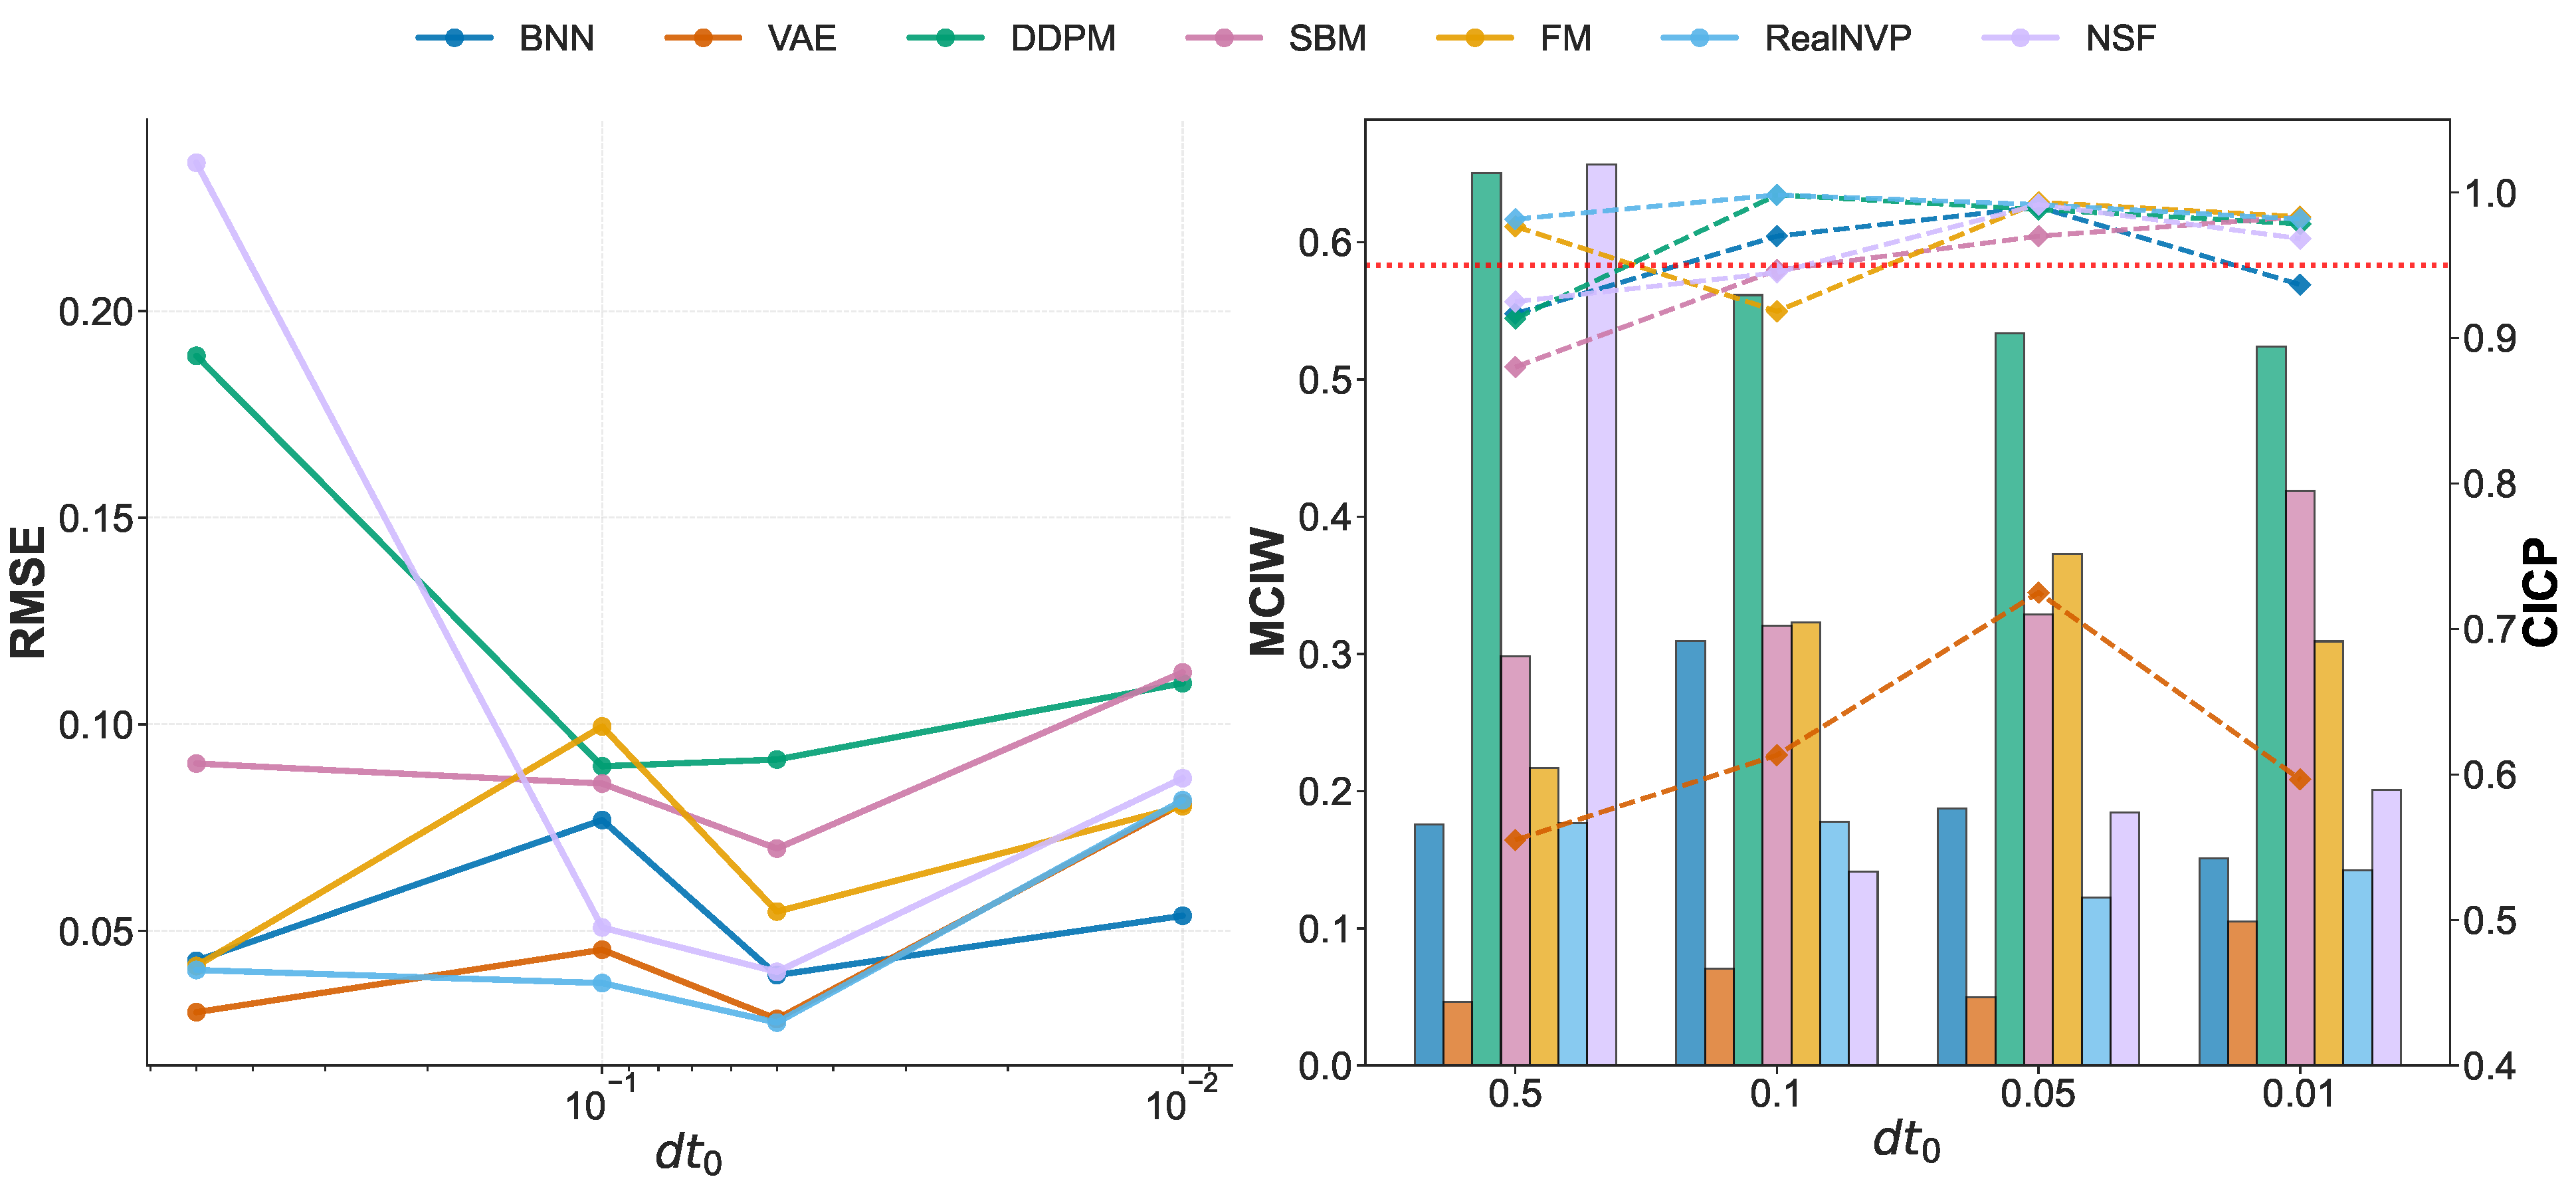
\includegraphics[width=\textwidth]{figures/curve_chart_sample.pdf}
    \caption[Performance Comparison w.r.t. Sample Efficiency]{Performance Benchmarking of Deep Bayesian Inference Methods under Varying Observation Densities. The left panel illustrates the predictive accuracy (RMSE) across time step $dt_0=[0.5, 0.1, 0.05, 0.01]$ plotted on a logarithmic scale where smaller $dt_0$ represents higher sampling density. The right panel provides a hybrid uncertainty analysis: the grouped bars indicate the MCIW (uncertainty precision), while the superimposed dashed lines represent the CICP (calibration reliability). The horizontal dotted line denotes the 95\% coverage target.}
    \label{fig:se_comp}
\end{figure}

The results in Figure \ref{fig:se_comp} characterize how the density of temporal observations impacts the posterior estimation. As the time step $dt_0$ decreases from $0.5\,s$ to $0.05\,s$, thereby increasing the total number of observations, all models show a consistent improvement in predictive accuracy, which can be attributed to the improved identifiability of the system dynamics. But the accuracy degrades at $dt_0=0.01\,s$ probably due to the inappropriate information extraction by the encoder, which is not designed for long time series. For a simple Mass-Spring-Damper system, $dt_0=0.05\,s$ already provides more than enough information to identify the parameters perfectly. Adding more points adds redundancy but no new constraints. This redundancy can lead to over-fitting in the latent space, where the model interprets numerical rounding errors or minor architectural biases as significant physical features. 

The accuracy of \ac{BNN}, \ac{RealNVP}, and \ac{VAE} is less sensitive to the sample efficiency. The higher RMSE at $dt_0=0.5\,s$ demonstrates that diffusion-based methods and \ac{NSF} requires more data than the other architectures. While almost all models reach accuracy peak at $dt_0=0.05\,s$, \ac{FM} prefers lower resolution of observation could result from that the vector field learning requires more differences in data samples. 

About uncertainty quantification demonstrated on the right panel in Figure \ref{fig:se_comp}, \ac{VAE} is overfitted with a very narrow confidence interval and inadequate coverage probability. In accordance with Bayesian theory, as the number of observations increases, the posterior distribution shrinks. In the regime of increasing data density from $dt_0=0.5\,s$ to $0.05\,s$, the models exhibit divergent uncertainty behaviors:
\begin{itemize}
    \item Consistent Posterior Shrinkage: \ac{DDPM} and \ac{RealNVP} demonstrate a clear shrinkage effect, where the MCIW drops consistently. This aligns with Bayesian expectations: as the number of observations increases, the likelihood becomes more peaked, forcing the posterior distribution to contract around the true parameters.
    \item Architectural Volatility: Other architectures show more complex trends. The MCIW of the \ac{BNN} initially increases before dropping, while \ac{NSF} exhibits a "decrease-then-rise" pattern. Most notably, \ac{FM} and \ac{SBM} show a paradoxical increase in MCIW (uncertainty width) as data density increases. This suggests that for these models, the increase in sequence length introduces numerical complexity or "perceived" contradictions in the latent space that temporarily outweigh the additional information provided by the higher sampling rate.
\end{itemize}
   
    
In terms of the reliability requirement, defined as a \ac{CICP} $\ge 0.95$, proves difficult to satisfy under sparse sampling. At $dt_0=0.5\,s$, only \ac{RealNVP} and \ac{FM} are successfully calibrated. This highlights the robustness of both architectures when dealing with sparse temporal trajectories. As data density improves to $dt_0=0.1\,s$, \ac{FM} temporarily drops out of the reliable regime, likely due to the aforementioned rise in its \ac{MCIW} not being perfectly aligned with its predictive accuracy. The performance peak occurs at $dt_0=0.05\,s$, where every model successfully satisfies the reliability requirement. This suggests that $0.05\,s$ is the optimal resolution for this system—providing sufficient information to identify the ODE parameters without reaching the point of numerical saturation. 

As sampling reaches the highest density $dt_0=0.01\,s$, the models encounter a breakdown in both accuracy and calibration:
\begin{itemize}
\item Divergent Uncertainty Trends: In this over-sampled regime, \ac{DDPM} and \ac{BNN} continue to shrink their MCIW further. However, for \ac{BNN}, this leads to a drop in CICP, indicating that the model is becoming overconfident. Its intervals are shrinking faster than its error, causing it to miss the ground truth.
\item Posterior Expansion: Conversely, \ac{SBM}, \ac{RealNVP}, and \ac{NSF} exhibit an increase in MCIW. This change in the posterior width is a defensive mechanism; as the models' RMSE increases due to the numerical difficulty of processing extremely high-frequency noise-free data, the models broaden their uncertainty bounds to maintain coverage.
\item Flow Matching Recovery: \ac{FM} reverses its previous trend and begins to drop in MCIW, suggesting it eventually finds a more stable numerical representation of the high-density data than the other flow variants.
\end{itemize}

The evaluation suggests that more observations do not always lead to better performance. \ac{RealNVP} is the most precise under sparse data, when ruling out the \ac{VAE}. \ac{BNN} is the most consistent at shrinking its bounds, suggesting that its variance measures the mathematical convergence of the weights, but not necessarily the "correctness" of the physical parameters. Notably, A pivot point in model reliability is observed at $dt_0=0.1\,s$, where \ac{SBM} and \ac{NSF} achieve perfect calibration, meeting the CICP target of exactly 0.95. Their paths to this threshold, however, are distinct: \ac{SBM} reaches the reliable regime through a corrective expansion of its posterior variance (increasing MCIW), while \ac{NSF} reaches it through efficient shrinkage, utilizing the increased temporal information to narrow its credible intervals while remaining perfectly on-target. At this mid-range resolution, these two models define the boundary of the reliable regime, whereas architectures like the \ac{BNN} and \ac{DDPM} remain under-calibrated despite the increased data density.

\paragraph{Linear Correlation}
When parameters are linearly correlated, the observations only constrain their ratio, rendering the individual parameters non-identifiable. While \acp{DGM} are capable of capturing these dependencies, the task is computationally harder than identifiable ones. The ill-posedness manifests as a manifold of equivalent solutions, making it difficult for optimization algorithms to distinguish between physically distinct systems that produce identical observations. When the correlation between $m$ and $k$ are fixed to be $k=10\cdot m$, the damping coefficient should also be proportional to the mass, i.e., $c\propto m$. The damping coefficient $c$ is related to the damping ratio $\zeta$ (which determines if the system is under-damped, critically damped, or over-damped) by the formula:
\begin{equation}
    c=2\zeta\sqrt{mk}.
\end{equation} 
Therefore, the following relation holds:
\begin{equation}
    c/m = 2\sqrt{10}\;\zeta.
\end{equation}
Figure \ref{fig:lc_comp} shows two identification examples of linear correlated parameters.
\begin{figure}[htp!]
    \centering
    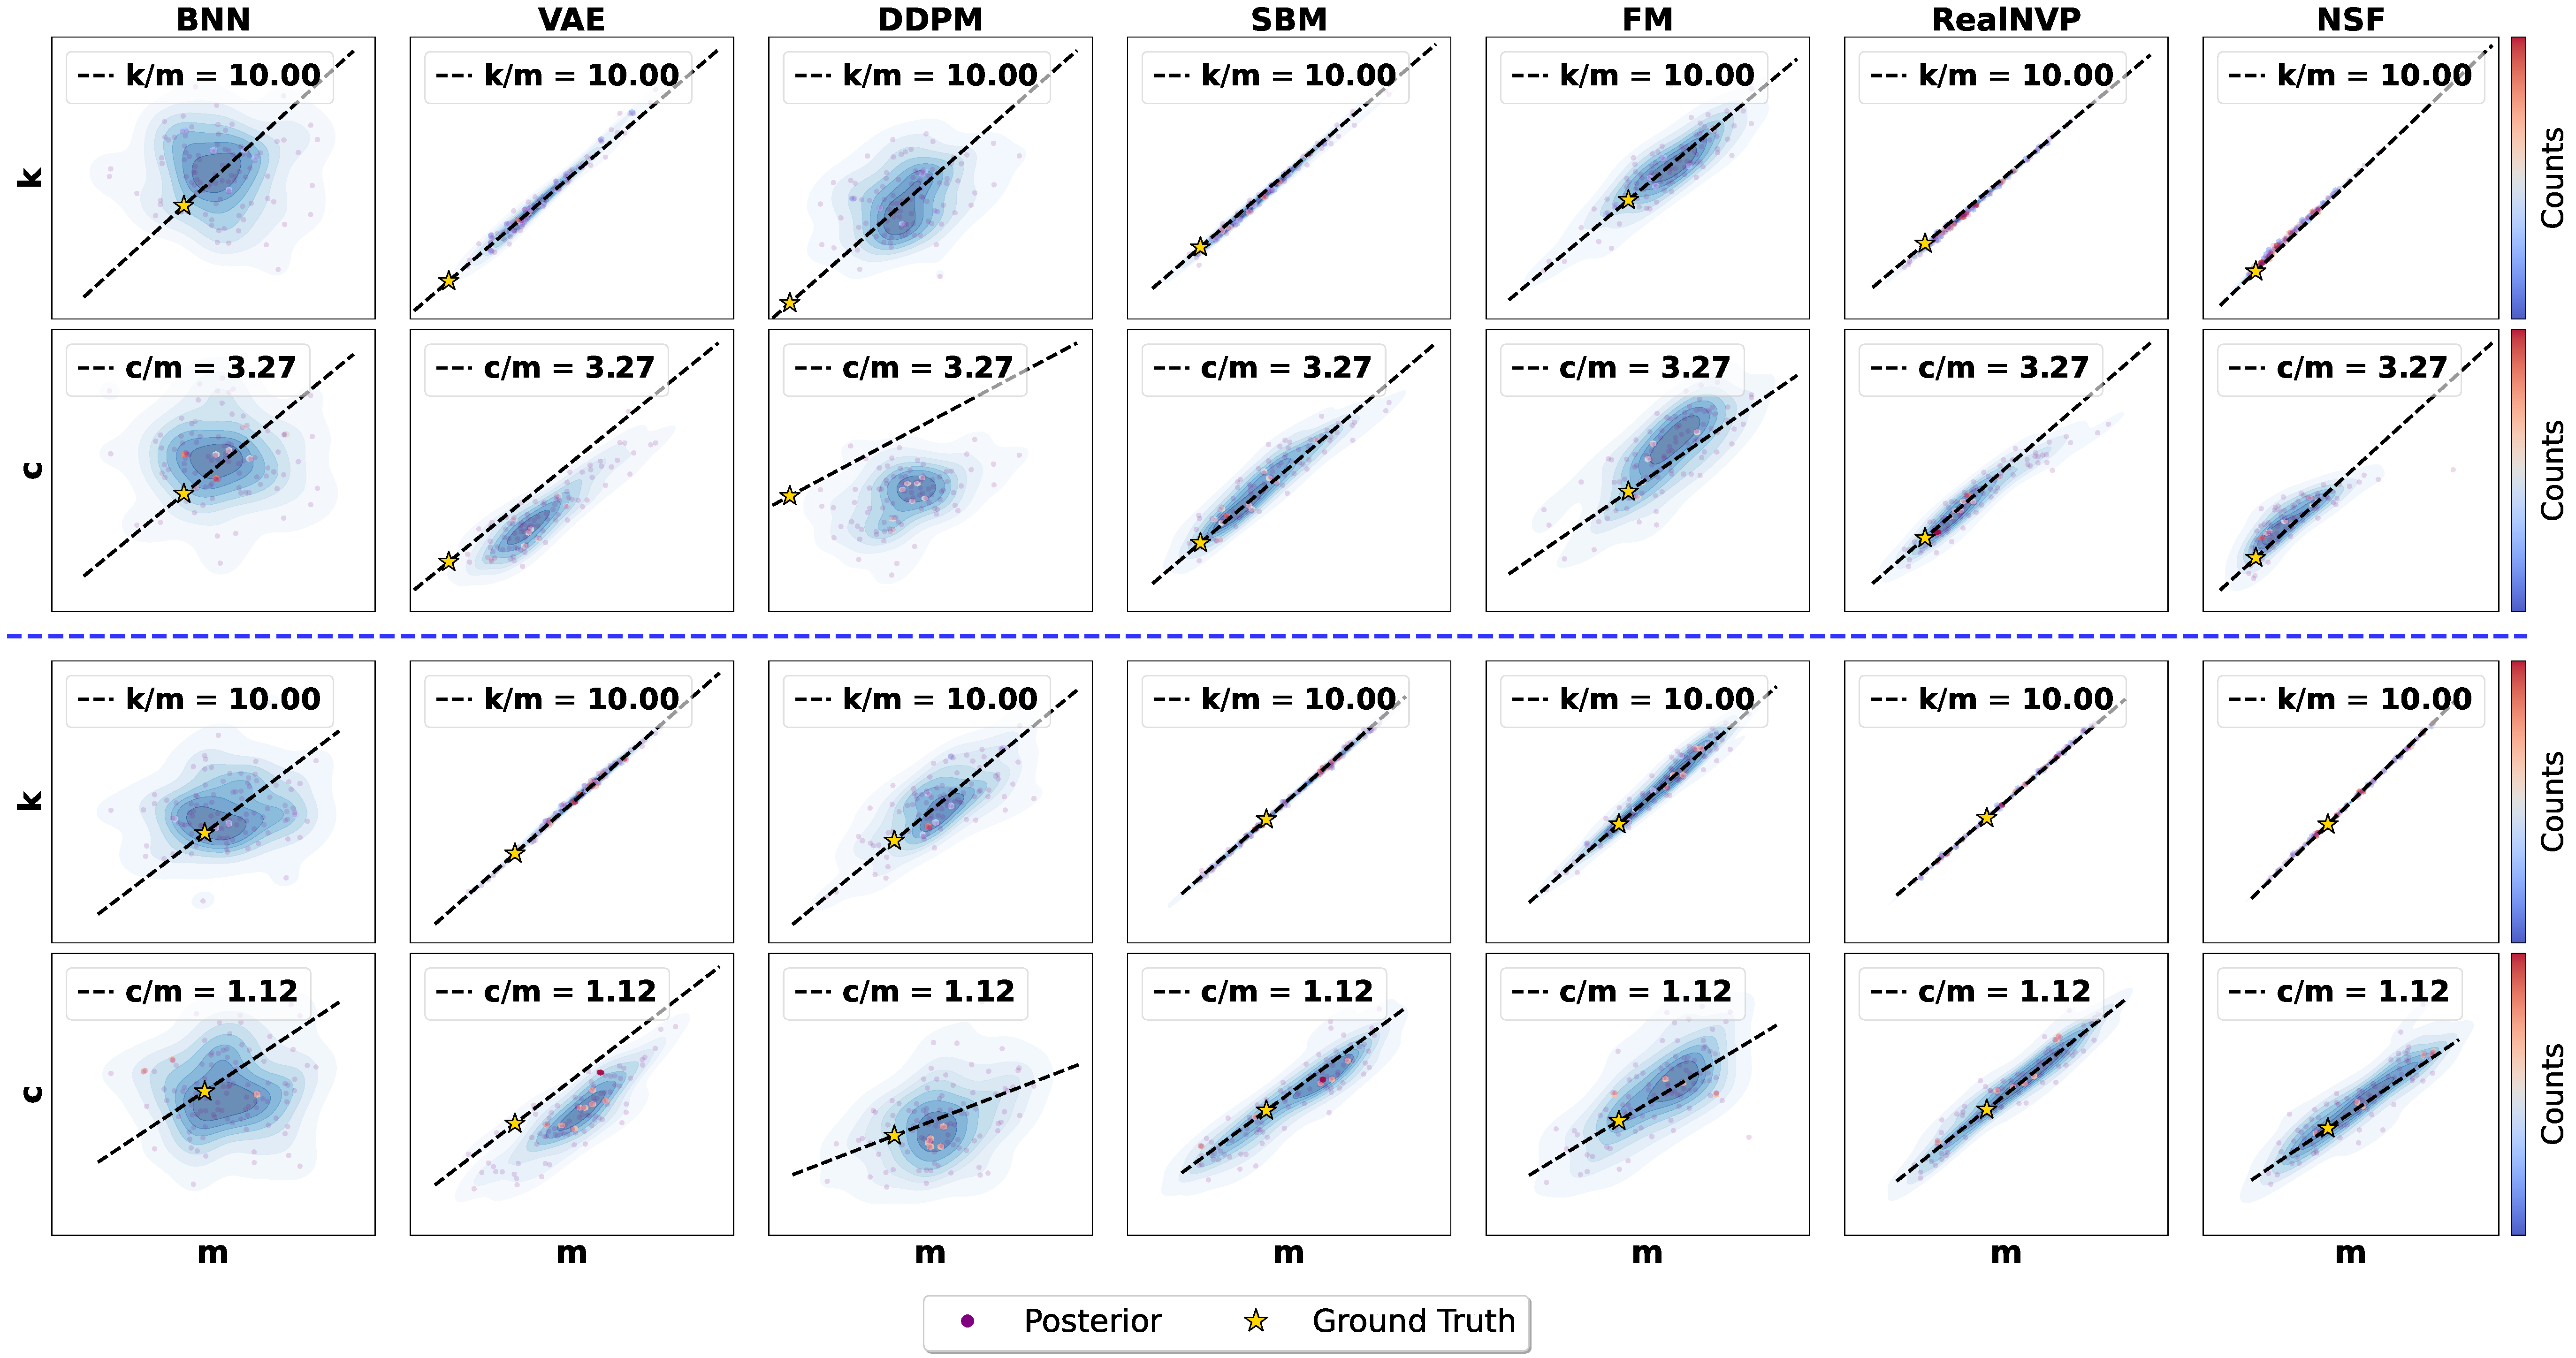
\includegraphics[width=\textwidth]{figures/model_comparison_grid_linear.pdf}
    \caption[Linear Correlation Comparison]{Comparative analysis of deep Bayesian inference architectures in identifying linearly correlated parameters. The $4\times7$ grid displays the joint posterior distributions for seven different models (columns) across two test scenarios (separated by a horizontal blue dashed line in the middle). Rows 1 and 3 visualize the $m-k$ correlation, while Rows 2 and 4 visualize the $m-c$ correlation. Within each sub-figure, the gold star represents the ground truth, and the black dashed line illustrates the theoretical linear constraint ($k/m$ or $c/m$). Individual posterior samples are plotted as purple points, overlaid on a logarithmic density heatmap where warm hues indicate regions of high probability mass. Note: To ensure high visibility of the posterior topology across models with varying precision, axis limits and density color-scales are individually optimized for each sub-figure. Each color map suits the whole row.}
    \label{fig:lc_comp}
\end{figure}

As illustrated in Figure \ref{fig:lc_comp}, the \ac{BNN} and \ac{DDPM} fail to capture the underlying dependencies, resulting in wide, uninformative posterior clouds that lack alignment with the physical constraints. While the \ac{VAE} recovers the $k/m$ correlation, it fails significantly on $c/m$, where the posterior mass is biased and poorly aligned with the diagonal line. In contrast, the remaining four methods demonstrate higher fidelity. 

Among the successful models, \ac{SBM} and the \ac{NF} architectures (\ac{RealNVP} and \ac{NSF}) show their superior capability in identifying and enforcing linear parameter correlations. Their $k/m$ estimates are tightly aligned with the theoretical diagonal, and their $c/m$ estimates manifest as narrow ellipses centered on the ground truth. On the other hand, \ac{FM} successfully captures the linear trend, but it exhibits noticeably higher variance compared to \ac{SBM}, \ac{RealNVP}, and \ac{NSF}, particularly in the $c/m$ correlations. This suggests that while \ac{FM} identifies the correlation, it is less precise in enforcing the constraint than other architectures.

Linear correlations represent a low-dimensional manifold within the parameter space. Figure \ref{fig:lc_comp} demonstrates that \acp{NF} (\ac{RealNVP}/\ac{NSF}) and \ac{SBM} are superior at manifold learning by effectively collapsing the posterior mass onto a line, whereas \ac{BNN} and \ac{DDPM} struggle to resolve such sharp constraints. Besides, the \ac{VAE}’s failure in the $c/m$ correlation is a classic symptom of posterior collapse or architectural under-fitting for specific parameter dimensions. 

The performance gap between the two diffusion models is particularly striking: \ac{SBM} exhibits a far greater capability for recovering precise physical constraints than \ac{DDPM}. Despite \ac{DDPM}'s established success in generating high-dimensional complex data, it fails to resolve the specific linear parameter correlations in this task.
Similarly, despite their theoretical proximity, \ac{FM} appears more dispersed than \ac{SBM}. This is primarily because \ac{FM} is a deterministic transport method that is more sensitive to cumulative approximation errors along the integration path, whereas the stochastic nature of \ac{SBM} provides a corrective mechanism through noise-driven sampling.

Within the \ac{NF} architectures, a notable distinction exists between \ac{RealNVP} and \ac{NSF} when we zoom in the $c/m$ figures. While both successfully identify the correlation, \ac{RealNVP} exhibits a higher degree of centralization along the diagonal correlation axes. While this leads to a narrower, line-like distribution with high precision, it also places the ground-truth (yellow star) at the extreme periphery of the high-density core. In contrast, \ac{NSF} estimates the density with higher variance, which is less desired in this case. 

\paragraph{Multimodal Distribution}
The ability to capture multimodal distributions is a key advantage of applying \acp{DGM} for Bayesian inference. Different \acp{DGM} exhibit different characteristics. Figure \ref{fig:mm_comp} illustrates these differences. As test scenarios, we consider two cases: one where the values of $k_1$ and $k_3$ are far apart (the first two samples), and another where they are close to each other (the last two samples).
\begin{figure}[htp!]
    \centering
    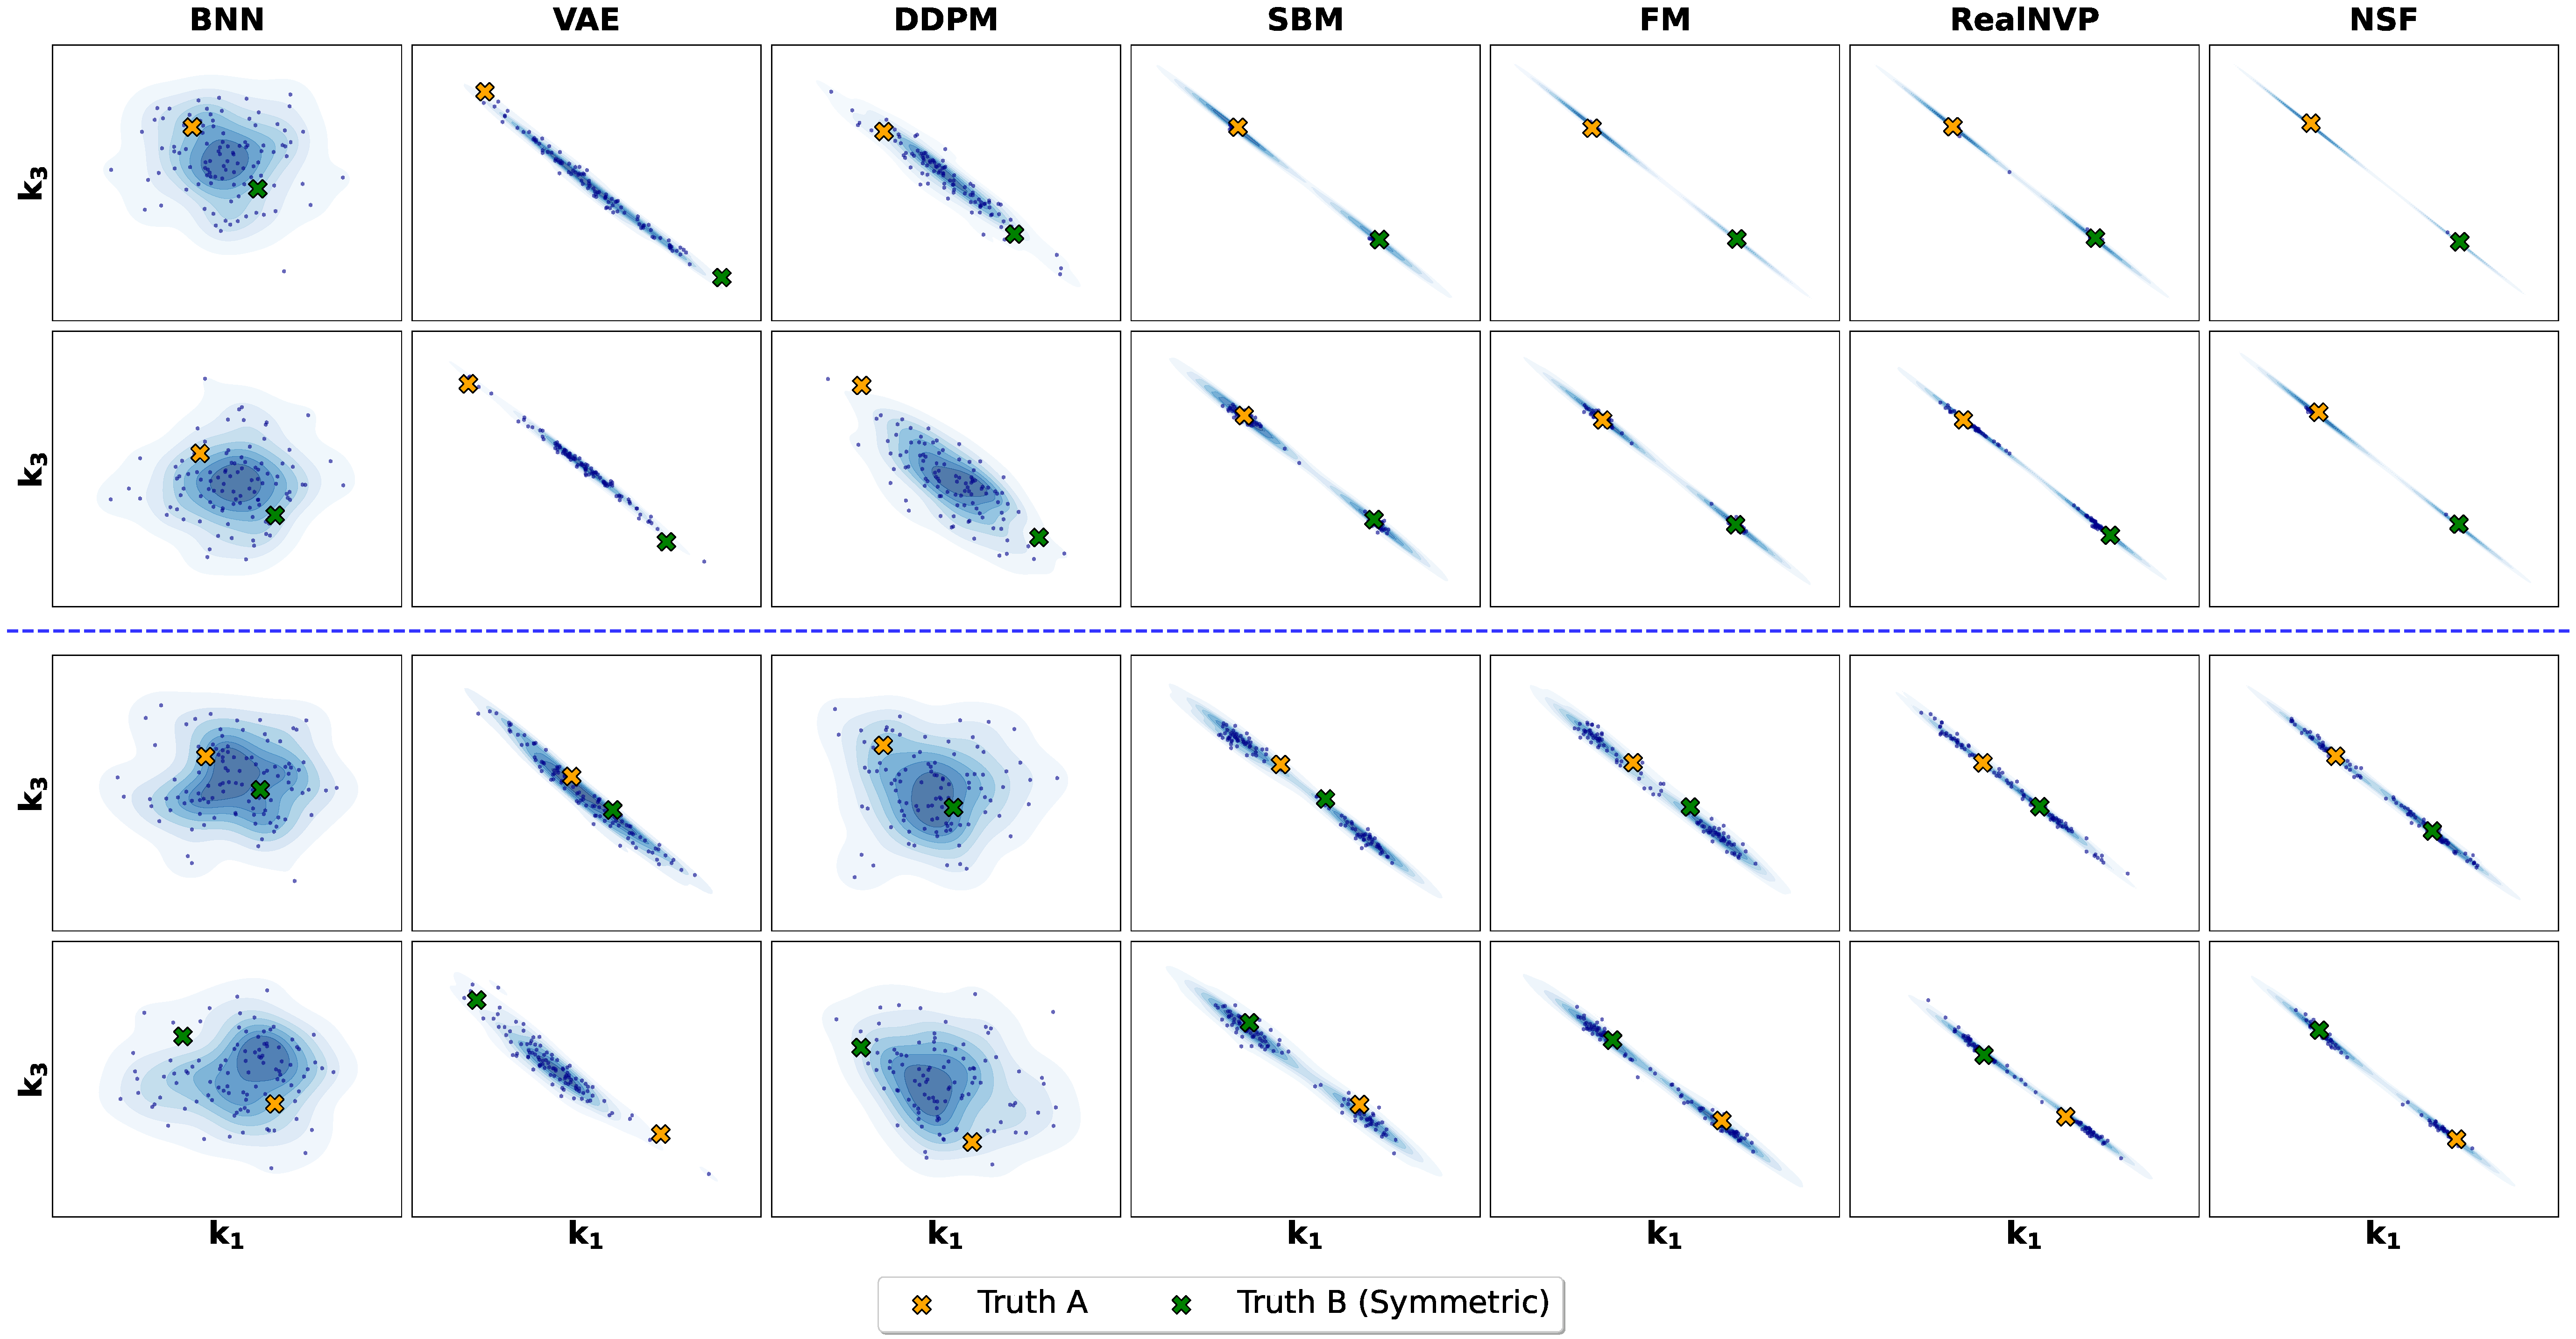
\includegraphics[width=\textwidth]{figures/model_comparison_grid_multi_modal.pdf}
    \caption[Multimodal Comparison]{Comparative evaluation of deep Bayesian architectures in recovering multimodal posterior distributions. The $4\times7$ grid displays the joint posterior of $k_1$ and $k_3$ for seven different models (columns) across four distinct test scenarios (rows). The top two rows represent scenarios with well-separated modes, while the bottom two rows represent scenarios with proximal (overlapping) modes (partitioned by a blue dashed line). Within each subplot, the orange cross denotes the target ground truth, while the green cross represents the symmetric ground truth (swapped $k_1$ and $k_3$ values), highlighting the models' ability to capture the inherent exchangeable symmetry of the parameter space. Blue contours represent the estimated posterior density. Note: To ensure high visibility of the posterior topology across models with varying precision, axis limits and density color-scales are individually optimized for each sub-figure.}
    \label{fig:mm_comp}
\end{figure}
 
As demonstrated in Figure \ref{fig:mm_comp}, there is a clear performance consistent with the linear correlation results. \ac{SBM}, \ac{FM}, \ac{NSF}, and \ac{RealNVP} significantly outperform \ac{BNN}, \ac{VAE}, and \ac{DDPM} in resolving the symmetric multimodal structure.
The \ac{BNN} produces broad, uninformative posterior clouds that fail to recognize any specific multimodal topology. The \ac{VAE} exhibits over-concentration onto narrow, biased ridges; in all these four scenarios, the ground truth and its symmetric counterpart lie entirely outside the high-density regions, indicating again, the posterior collapse. \ac{DDPM} successfully resolves the two distinct modes only in the first scenario (Row 1), but degrades into a single diffuse, biased cluster in the remaining test cases.

In contrast, \ac{SBM}, \ac{FM}, and \ac{NSF} demonstrate superior multimodal recovery. In the well-separated scenarios (top two rows), they clearly resolve two distinct high-probability peaks. As the modes become proximal (bottom two rows), these models transition to a single elongated density region that embraces both ground truth points. While \ac{RealNVP} successfully identifies both modes, it produces extremely thin, line-like distributions with collapsed variance. This suggests that the \ac{RealNVP} has failed to capture the full uncertainty of the posterior due to its limited expressiveness. Instead, it collapses onto a lower-dimensional manifold.

There is a clear phase transition in model behavior between Row 2 and Row 3. All successful models transition from disjoint bimodal to continuous unimodal as the parameter modes move closer together. This shows that the models are not just memorizing two points, but are actually learning the underlying likelihood surface. Comparing \ac{SBM} and \ac{FM} reveals that while both use related ODE/SDE-based sampling, \ac{SBM} produces a much crisper, tighter posterior. \ac{FM} appears more noisy and diffused, suggesting that for high-precision physical parameter identification, score-based objectives might offer better convergence to the true posterior manifold than standard flow-matching. The \ac{NSF} appears to be the most balanced architecture. It avoids the extreme thinness of \ac{RealNVP} while maintaining the high precision and multimodal resolution.

\subsection{Relationship Between Bayesian Inference and Sensitivity Analysis}
Previous experiments applying mass-spring-damper models demonstrate that Bayesian inference is intrinsically linked to parameter identifiability. Our findings indicate that spring constants converge rapidly during training, which will be further elucidated through sensitivity analysis. Conversely, linearly correlated parameters lack unique identification, and in symmetric coupled models, individual spring constants become indistinguishable. These varying levels of identifiability can be rigorously analyzed through \ac{SA}, which studies how uncertainty in the output of a mathematical model can be partitioned and allocated to different sources of uncertainty in its inputs. This framework aligns naturally with the objectives of amortized Bayesian inference. For purely data-driven methods, \ac{SA} provides essential insights into the physical model and practical training suggestions: weakly identifiable or correlated parameters that require additional observational data for resolution.

Unlike local \ac{SA}, which examines instantaneous changes in output relative to specific parameter perturbations, our research focuses on total trajectories, necessitating a global \ac{SA}. A common approach for global \ac{SA} is the Sobol' index, which is a variance-based method that decomposes the total output variance into contributions from individual parameters and their interactions. For a model $f$ with inputs $X_1, \ldots, X_d$ and the output $Y$, the total variance of the model output is:
\begin{equation}
    Var(Y) = \sum_i V_i + \sum_{i<j} V_{ij} + \cdots + V_{1,2,\ldots,d}.
\end{equation}
The first-order Sobol' index $S^1_i$ measures the contribution of a single parameter $X_i$ to the output variance, which can be regarded as the main effect. It is given by:
\begin{equation}
    S^1_i = \frac{V_i}{Var(Y)}\quad V_i=Var_{X_i}[E_{\boldsymbol{X}_{\sim i}}(Y|X_i)].
\end{equation}
The total Sobol' index accounts for the total contribution of a parameter to the output variance, including both its main effect and all higher-order interactions with other parameters. The total Sobol' index of $X_i$ is
\begin{equation}
    S^T_i = \frac{Var_{\boldsymbol{X}_{\sim i}}[E_{X_i}(Y|\boldsymbol{X}_{\sim i})]}{Var(Y)}.
\end{equation}

Another key issue of using variance-based \ac{SA} is to sample the parameter space efficiently. The standard random sampling often creates clusters or gaps in the parameter space. Instead, Sobol' sequences are applied, which are low-discrepancy sequences. For the sake of stability, a larger number of samples should be set.

By comparing these two indices, we can diagnose the structural complexity of the mass-spring-damper system. For instance, a parameter with a high total Sobol' index but a low first-order Sobol' index indicates that while the parameter is influential, its effect is primarily driven by interactions with other components of the model. The linear correlation and multimodality cases are supposed to have zero first-order Sobol' indices and one total Sobol' indices. 
If a parameter exhibits a total Sobol' index near zero, it suggests that the model output is insensitive to that parameter across its entire prior range. Such parameters are unidentifiable under the provided observed data. 

Ultimately, integrating global \ac{SA} into the amortized Bayesian workflow allows us to preventively identify "blind spots" in the model. By detecting parameters with low sensitivity or high correlation, we can strategically focus on data collection efforts or reparameterize the model to ensure that the posterior distributions are well-defined and physically meaningful. When parameters exhibit significantly different levels of identifiability, a sensitivity-guided iterative identification strategy is recommended. In such cases, strongly identifiable parameters (those with high $S^1_i$ values, like the primary spring constants) should be identified first to stabilize the model. Once these dominant parameters are constrained, the remaining weakly identifiable or highly correlated parameters can be addressed in subsequent stages by adaptation of observational data or by refining the prior distributions. This hierarchical approach prevents the variance of dominant parameters from obscuring the signals of secondary parameters, ensuring a more robust and physically meaningful calibration of the complex system.

The sensitivity of parameters also reflects the convergence speed of training deep Bayesian inference models as well. Taking a closer look at the mass-spring-damper model with external force, we get very close first-order and total-order indices, i.e., $S^1_m=0.07, S^1_k=0.88, S^1_c=0.03$ and $S^T_m=0.07, S^T_k=0.89, S^T_c=0.05$. It suggests for the single-degree-of-freedom system under external excitation, the stiffness parameter $k$ dominates the system response and there is hardly no parametric interaction. This means the model is effectively additive in the chosen parameter ranges. From an identifiability perspective, the $k$ should be much easier to estimate than the other two parameters. 
\begin{figure}[htbp]
    \centering

    \begin{subfigure}[b]{0.48\textwidth}
        \centering
        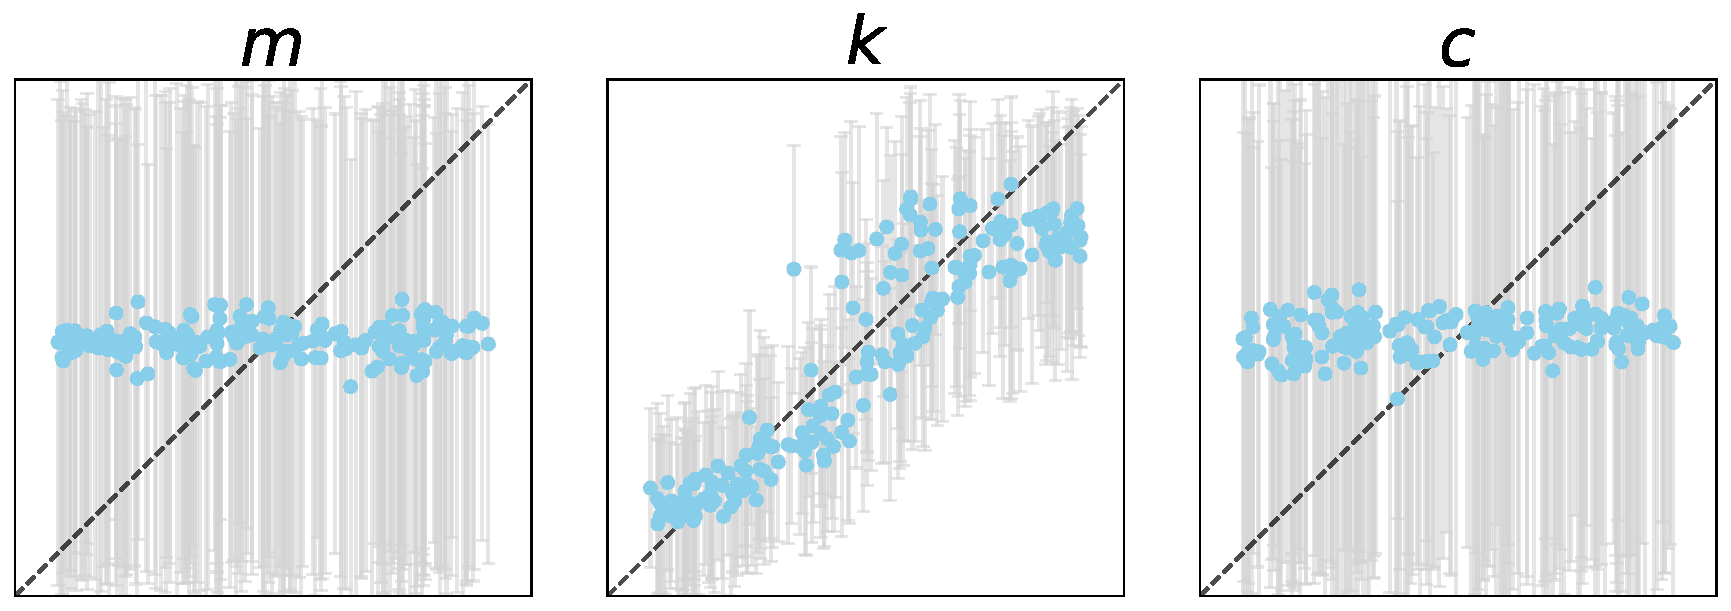
\includegraphics[width=\textwidth]{figures/RealNVP_mass_spring_damper_0.05_1.0_force_29.pdf}
        \caption{Epoch=29}
        \label{fig:sa_01}
    \end{subfigure}
    \hfill
    \begin{subfigure}[b]{0.48\textwidth}
        \centering
        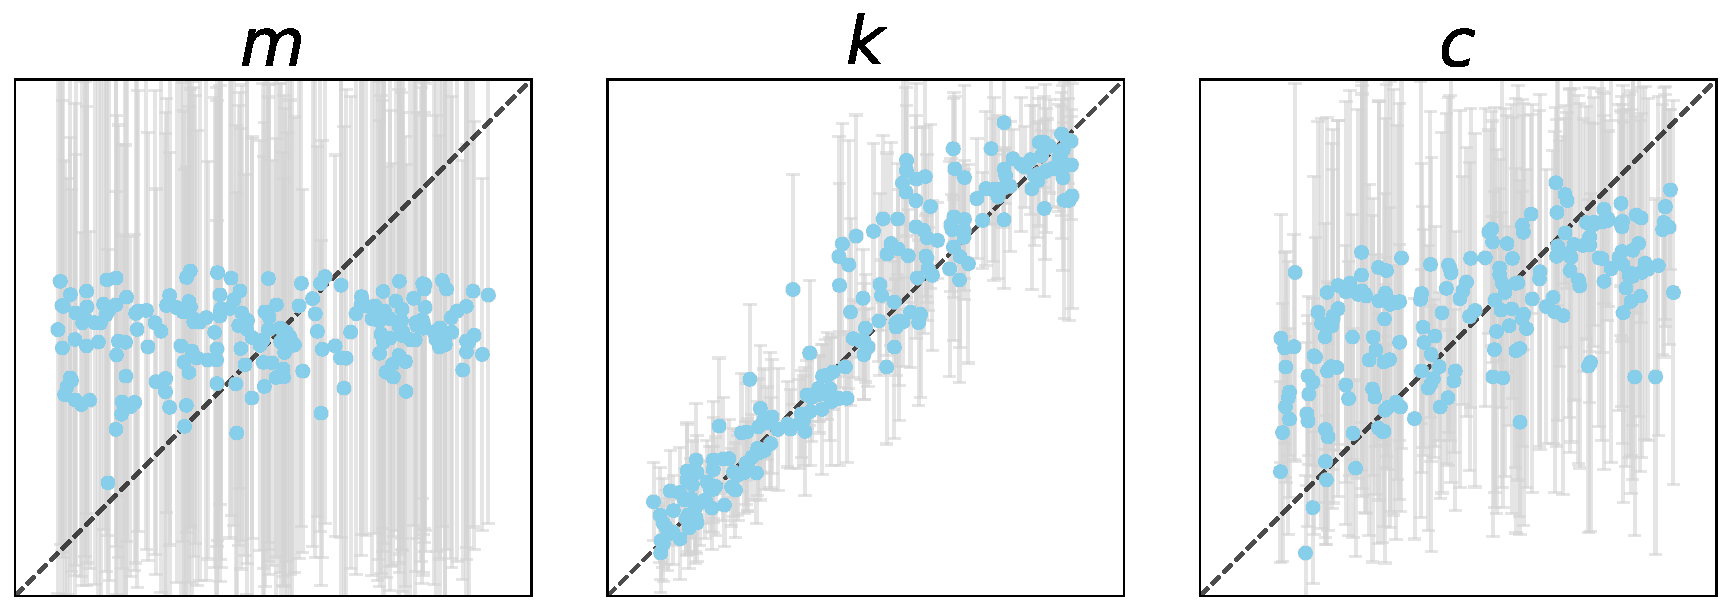
\includegraphics[width=\textwidth]{figures/RealNVP_mass_spring_damper_0.05_1.0_force_258.pdf}
        \caption{Epoch=258}
        \label{fig:sa_02}
    \end{subfigure}

    \begin{subfigure}[b]{0.48\textwidth}
        \centering
        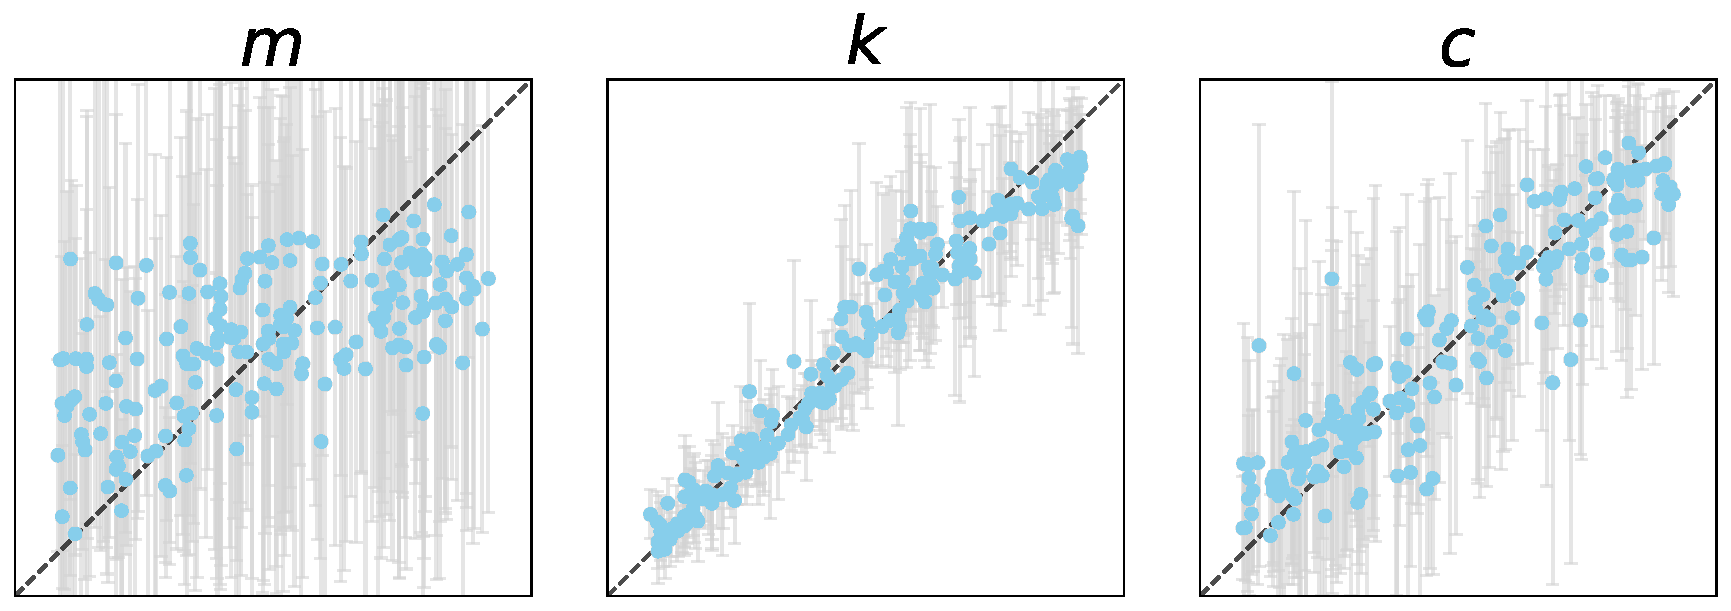
\includegraphics[width=\textwidth]{figures/RealNVP_mass_spring_damper_0.05_1.0_force_393.pdf}
        \caption{Epoch=393}
        \label{fig:sa_03}
    \end{subfigure}
    \hfill
    \begin{subfigure}[b]{0.48\textwidth}
        \centering
        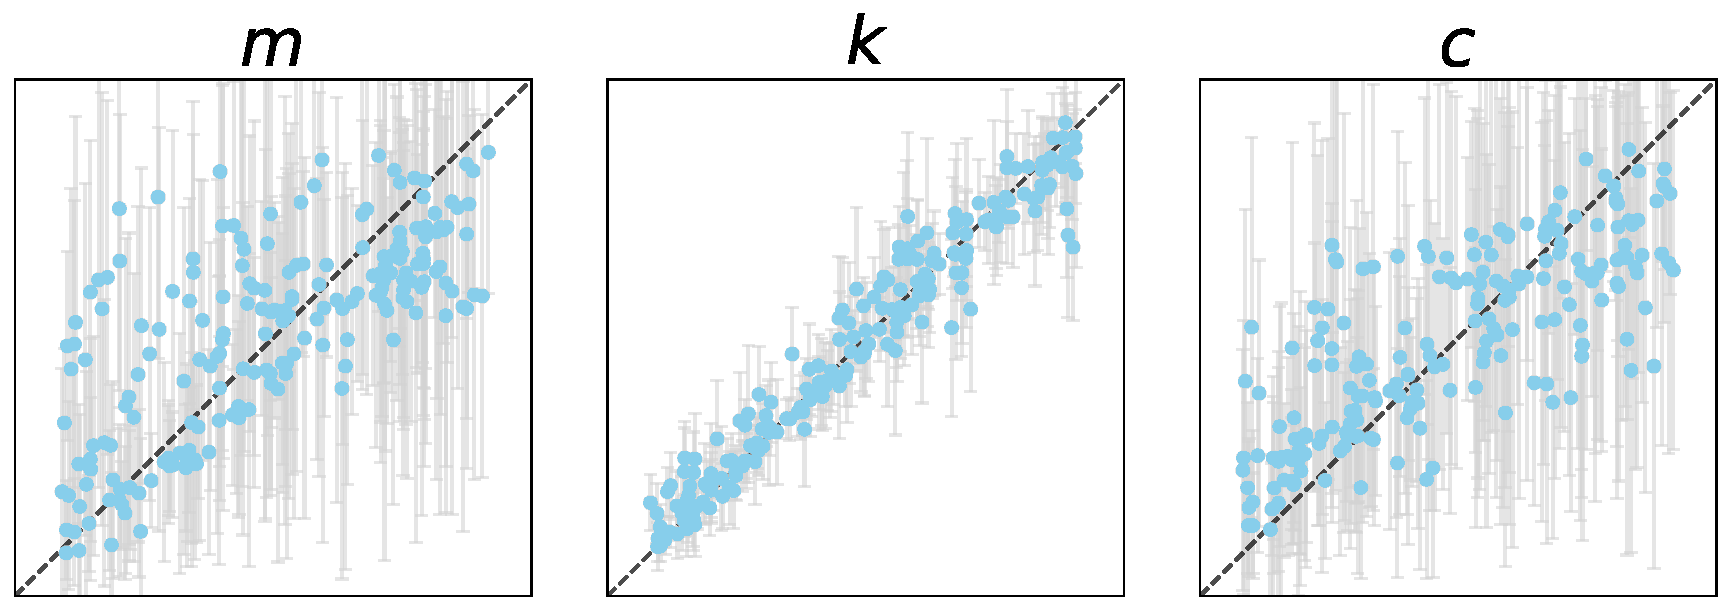
\includegraphics[width=\textwidth]{figures/RealNVP_mass_spring_damper_0.05_1.0_force_951.pdf}
        \caption{Epoch=951}
        \label{fig:sa_04}
    \end{subfigure}

    \caption[Convergence Speed \& Sensitivity Analysis]{Parameter identification results of \ac{RealNVP} at the early training stages. The figures show the estimation results of parameters $m,k,c$. The horizontal axis represents the ground truth, while the vertical shows the estimated values. The perfect convergence is demonstrated by the diagonal dashed line.}
    \label{fig:sa_speed}
\end{figure}

Figure \ref{fig:sa_speed} illustrates the convergence behavior of the three parameters during the early stages of training. By the 29th epoch, the stiffness $k$ begins to converge toward the diagonal parity line, whereas the other two parameters remain unresolved, centered at the mean of their respective ranges. At the 258th epoch, $c$ begins to show a slight tendency toward convergence, while $k$ is further refined; however, $m$ shows no significant improvement. By the 393rd epoch, $m$ also begins to converge. Finally, at the 951st epoch, $m$ and $c$ reach a similar level of accuracy, while the estimate for $k$ continues to improve. This development reflects the sensitivity of parameters. It is worth to note that faster convergence of $c$ than $m$ results from the larger data range of $c$. And the convergence speed of both parameters synchronizes at the last. 

\begin{figure}[htbp]
    \centering
    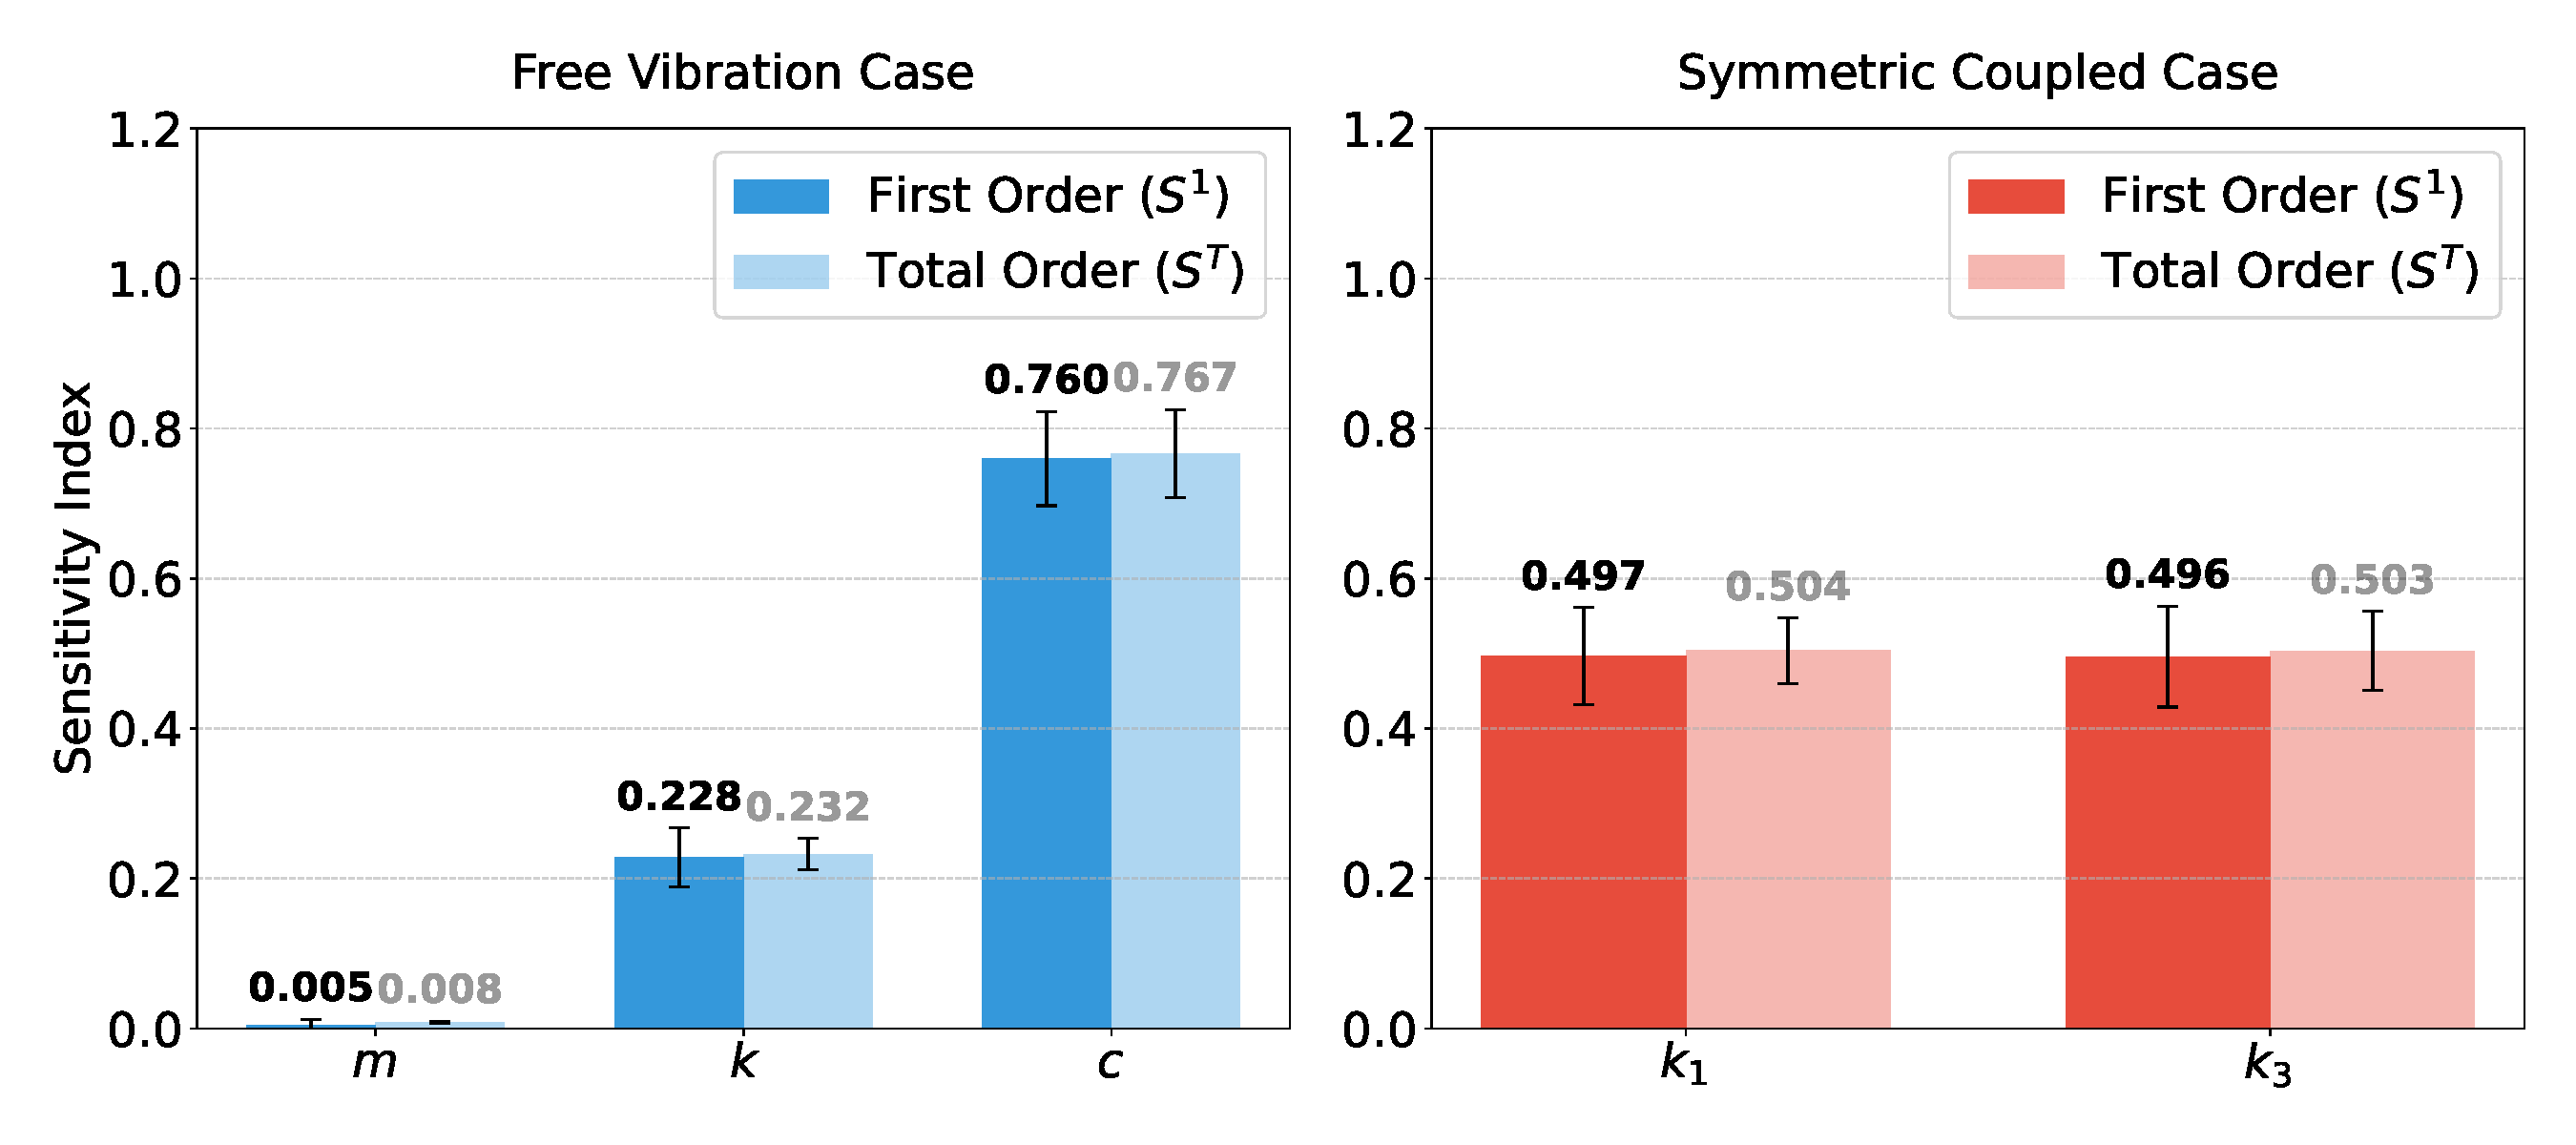
\includegraphics[width=0.9\textwidth]{figures/sensitivity_analysis_linear_coupled.pdf}
    \caption[Global Sensitivity Analysis of Free-Vibration and Symmetric Coupled Mass-Spring-Models]{Global \ac{SA} comparison in free-vibration and symmetric coupled mass-spring-damper systems. The bar charts display the first-order ($S^1$) and total-order ($S^T$) Sobol’ indices, with error bars representing the 95\% confidence interval. (Left) In the free-vibration case, the parameters $m,k,c$ are highly differently sensitive. (Right) In the symmetric coupled two-mass system, $k_1$ and $k_3$ exhibit nearly identical sensitivity.}
    \label{fig:sa_l_c}
\end{figure}

Figure \ref{fig:sa_l_c} compares the sensitivity analysis of the free and coupled mass-spring-models. In the free-vibration case, the external force is removed. The behavior of the mass-spring-model is heavily influenced by how fast the energy loses, which is caused by the damping $c$. The global \ac{SA} of the free-vibration system reveals a clear hierarchy of parameter identifiability. The damping coefficient  $c$ dominates the output variance ($S^T_c=0.767$), followed by the stiffness $k$ ($S^T_k=0.232$), and the mass $m$ exhibits negligible sensitivity ($S^T_m=0.008$). Furthermore, the near-equality of $S^1$ and $S^T$ across all parameters indicates a lack of higher-order interactions. This suggests $m$ is weakly identifiable, whereas the other two parameters can be identified independently. 

The global \ac{SA} of the symmetric coupled two-mass system reveals a perfect parity between the boundary stiffness parameters. Both $k_1$ and $k_3$ exhibit nearly identical first-order ($S^1\approx 0.496$) and total-order ($S^T\approx 0.503$) indices. The near-unity sum of their first-order indices ($S_{k_1}+S_{k_3}\approx 1$) suggests that these two parameters account for almost the entire variance of the system's dynamic response, with negligible higher-order interactions ($S^T-S^1<0.01$). From an identifiability perspective, this symmetry presents a unique challenge for Bayesian inference. While the high sensitivity ensures that the parameters will converge quickly away from the prior mean, the identical nature of their influence results in a bimodal posterior distribution. This confirms the indistinguishability and multimodality: the amortized inference model can identify the required stiffness levels but cannot uniquely assign them to $k_1$ or $k_3$ without additional asymmetric constraints or localized observations.

\subsection{When Does the Framework Fail?}
From the previous sections, we have known the framework frequently struggles with posterior identifiability; specifically, when the system exhibits multimodality, generative models may fail to resolve disjoint parameter regimes. Apart from identifiability, the efficacy of amortized Bayesian inference via deep generative models is intrinsically tied to the fidelity of the latent representations extracted by the condition network. This framework encounters significant bottlenecks under three primary conditions. First, in the presence of high-dimensional, noisy, or highly stochastic time-series data, the condition network often fails to distill sufficient summary statistics, leading to information loss. Second, the framework is susceptible to model misspecification. When a discrepancy exists between the training simulator and real-world dynamics (the 'sim-to-real gap'), the amortized posterior yields biased and poorly calibrated estimates. Third, the framework fails to generalize to parameter ranges outsized its training boundaries, even if the underlying physics remain the same. 

We evaluate the robustness of \acp{NF} (including \ac{FM}, \ac{RealNVP}, and \ac{NSF}) by subjecting the framework to the following stress-test scenarios:
\begin{itemize}
\item Information Extraction Bottlenecks: Increasing observational noise to assess the limits of the condition network's feature extraction.
\item Structural Misspecification: Evaluating models trained on linear dynamics against data generated from non-linear physical systems.
\item \ac{OOD} Generalization: Testing the framework on parameter ranges that lie outside the support of the training prior.
\end{itemize}

\subsection{Stochastic Normalizing Flows}
Normalizing flows, including flow matching, are deterministic by design, which enables precise and efficient density estimation. However, in practice this deterministic structure can limit their ability to fully capture complex, highly multimodal target distributions, especially when model capacity or data are limited. One way to alleviate this limitation is to combine normalizing flows with \ac{MCMC} methods. In such hybrid approaches, the normalizing flow serves as an expressive proposal or initialization mechanism, while \ac{MCMC} refines the samples by enforcing consistency with the true posterior through its accept–reject mechanism or transition kernel. The stochastic exploration of \ac{MCMC} improves mode coverage and helps the overall system discover and accurately represent multiple modes that might be underrepresented by the deterministic flow alone. Moreover, by repeatedly evaluating the forward dynamics within the \ac{MCMC} procedure, the method can better discriminate between parameter configurations that produce similar noisy observations, thereby improving parameter identifiability under measurement noise.

\citeauthor{wu2020stochasticnormalizingflows} \citeyearpar{wu2020stochasticnormalizingflows} proposed to construct \acp{SNF} by alternating a sequence of deterministic \acp{INN} and stochastic \ac{MCMC} sampling layers (INN - MCMC - $\cdots$ - INN - MCMC). \citeauthor{Hagemann_2022} \citeyearpar{Hagemann_2022} provided theoretical foundation for stochastic normalizing flows and proved their consistency to \acp{CNF} for solving inverse problems. An \ac{SNF} is a pair of Markov chains of random variables $((U_0, \ldots, U_T), (V_T, \ldots, V_0))$. The transformation between two adjacent variables is either a deterministic \ac{INN} block or a stochastic \ac{MCMC} sampling layer. Denoting the process $(U_t)_{t=0}^T$ as the forward process, $U_0$ represents the data and $U_T$ is trained to follow a standard normal distribution. Conversely, in the inverse process $(V_t)_{t=0}^T$, $V_T$ is sampled from the standard normal distribution and $V_0$ follows the target density. Because both processes are Markov chains, the transformations can be written as conditional distributions, where each state depends only on its immediate predecessor. We denote the transformations in the forward process by $\mathcal{T}_t = P(U_t \mid U_{t-1})$ and those in the inverse process by $\mathcal{T}_t^{-1} = P(V_{t-1} \mid V_t)$. An illustration of such an \ac{SNF} architecture is shown in Figure \ref{fig:snf}.
\begin{figure}[htp!]
    \centering
    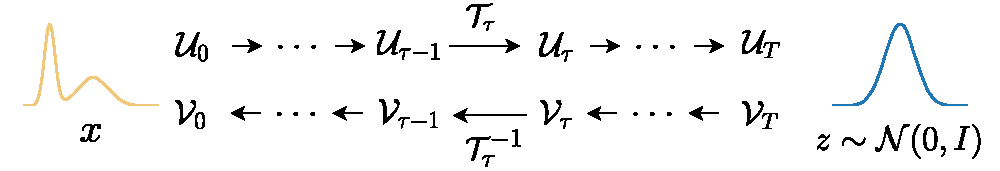
\includegraphics[width=0.9\textwidth]{figures/SNF.pdf}
    \caption[SNF Architecture]{ The architecture of an SNF.}
    \label{fig:snf}
\end{figure}

Unlike \acp{CNF}, for which the objective function is minimizing the KL-divergence between the learnt and target density, the objective function for training an \ac{SNF} is to minimize the difference of the joint probabilities between the forward and inverse processes. We define the joint probability of forward process as $p_\theta(u_{0:T})=p_X(u_0)\Pi_{t=1}^{T}p_\theta(u_t|u_{t-1})$, while the inverse process as $q_\theta(v_{0:T})=p_Z(v_T)\Pi_{t=1}^{T}q_\theta(v_{t-1}|v_{t})$. Same as \acp{CNF}, the objective function is trained in the forward direction.
\begin{multline}
\mathcal{L}_{SNF}(\theta)=D_{\text{KL}}(p_\theta(u_{0:T})||q_\theta(v_{0:T}))=\mathbb{E}_{u_{0:T}\sim p_\theta}[\log p_\theta(u_{0:T})-\log q_\theta(v_{0:T})]\\
=\mathbb{E}_{u_{0:T}\sim p_\theta}[-\log p_Z(u_T)+\log p_X(u_0)+\sum_{t=1}^{T}\log \frac{p_\theta(u_{t}|u_{t-1})}{q_\theta(u_{t-1}|u_{t})}].
\end{multline}
The critical point is the calculation of the term $\left[p_\theta(u_{t}|u_{t-1})/q_\theta(u_{t-1}|u_{t})\right]$.
\begin{itemize}
    \item For a deterministic transformation, the term is equivalent to the change of variable, which is given by:
    \begin{equation}
        \frac{p_\theta(u_{t}|u_{t-1})}{q_\theta(u_{t-1}|u_{t})} = \frac{du_{t-1}}{du_{t}} = -\log \det \left|J_f(u_{t-1})\right|.
    \end{equation}
    \item For a stochastic transformation, the term is the KL-divergence, measuring how well the backward kernel inverts the forward one at each step. The stochastic transformation is supposed to be invertible and has to fulfill the detailed balance condition with respect to some density $p_t$, which is given by:
    \begin{equation}
        p_t(u_t)q_\theta(u_{t-1}|u_t) = p_{t}(u_{t-1})p_\theta(u_t|u_{t-1}).
    \end{equation}
    The density $p_t$ is the target density of the stochastic layer at the $t$-th step. It is chosen to be an interpolation between $p_Z$ and $p_X$, which is given by:
    \begin{equation}
        p_t = c \cdot p_Z^{t/T} \cdot p_X^{(T-t)/T}.
    \end{equation}
    The parameter $c$ is a normalizing constant.

    For computational efficiency, the stochastic transformation is chosen to be an \ac{MALA} (See in Section\ref{sec:MALA}) kernel. Then, the term $\left[p_\theta(u_{t}|u_{t-1})/q_\theta(u_{t-1}|u_{t})\right]$ is given by:
    \begin{equation}
        \frac{p_\theta(u_{t}|u_{t-1})}{q_\theta(u_{t-1}|u_{t})} = \frac{p_t(u_{t})}{p_t(u_{t-1})} = \exp\left(-\frac{1}{2\tau}(\left\|\eta_t\right\|^2_2-\left\|\tilde{\eta}_t\right\|^2_2)\right),
    \end{equation}
    where 
    \begin{equation}
        \eta_t = u_t-u_{t-1}+\frac{\sqrt{\tau}}{2}\nabla E_t(u_{t-1}), \quad \tilde{\eta}_t = u_{t-1} -u_t+\frac{\sqrt{\tau}}{2}\nabla E_t(u_{t}).
    \end{equation}
\end{itemize}

% MALA different places
% multimodal
% noisy case


